% !Mode:: "TeX:UTF-8"
% pages/appendix.tex
%%%--- “附录” --- %%%%%%%%%%%%%%%%%

\cleardoublepage\phantomsection
\titleformat{\chapter}{\centering\heiti\bfseries\zihao{3}}{附录\thechapter}{1em}{}
\titlespacing{\chapter}{0pt}{-1em}{1em}

\renewcommand{\thechapter}{\arabic{chapter}} % 改为阿拉伯数字
\newcommand{\appendixnumbering}{%
  \renewcommand{\thechapter}{\arabic{chapter}}% 强制附录使用 1,2,3...
  \setcounter{chapter}{0}% 从 1 开始编号
}
\renewcommand{\chaptermark}[1]{%
  \markboth{附录~\thechapter\quad #1}{}%
}

\makeatletter
\patchcmd{\appendix}{\setcounter{chapter}{0}}{\appendixnumbering}{}{}
\makeatother

\appendix
\appendixnumbering
\addcontentsline{toc}{chapter}{附录1}
\addtocontents{toc}{\protect\setcounter{tocdepth}{-1}} % 临时禁止加入目录
\chapter{}

这是一个关于数字电压表的电路原理图。这是一个关于数字电压表的电路原理图。这是一个关于数字电压表的电路原理图。这是一个关于数字电压表的电路原理图。这是一个关于数字电压表的电路原理图。
  
\begin{figure}[H]
  \centering
  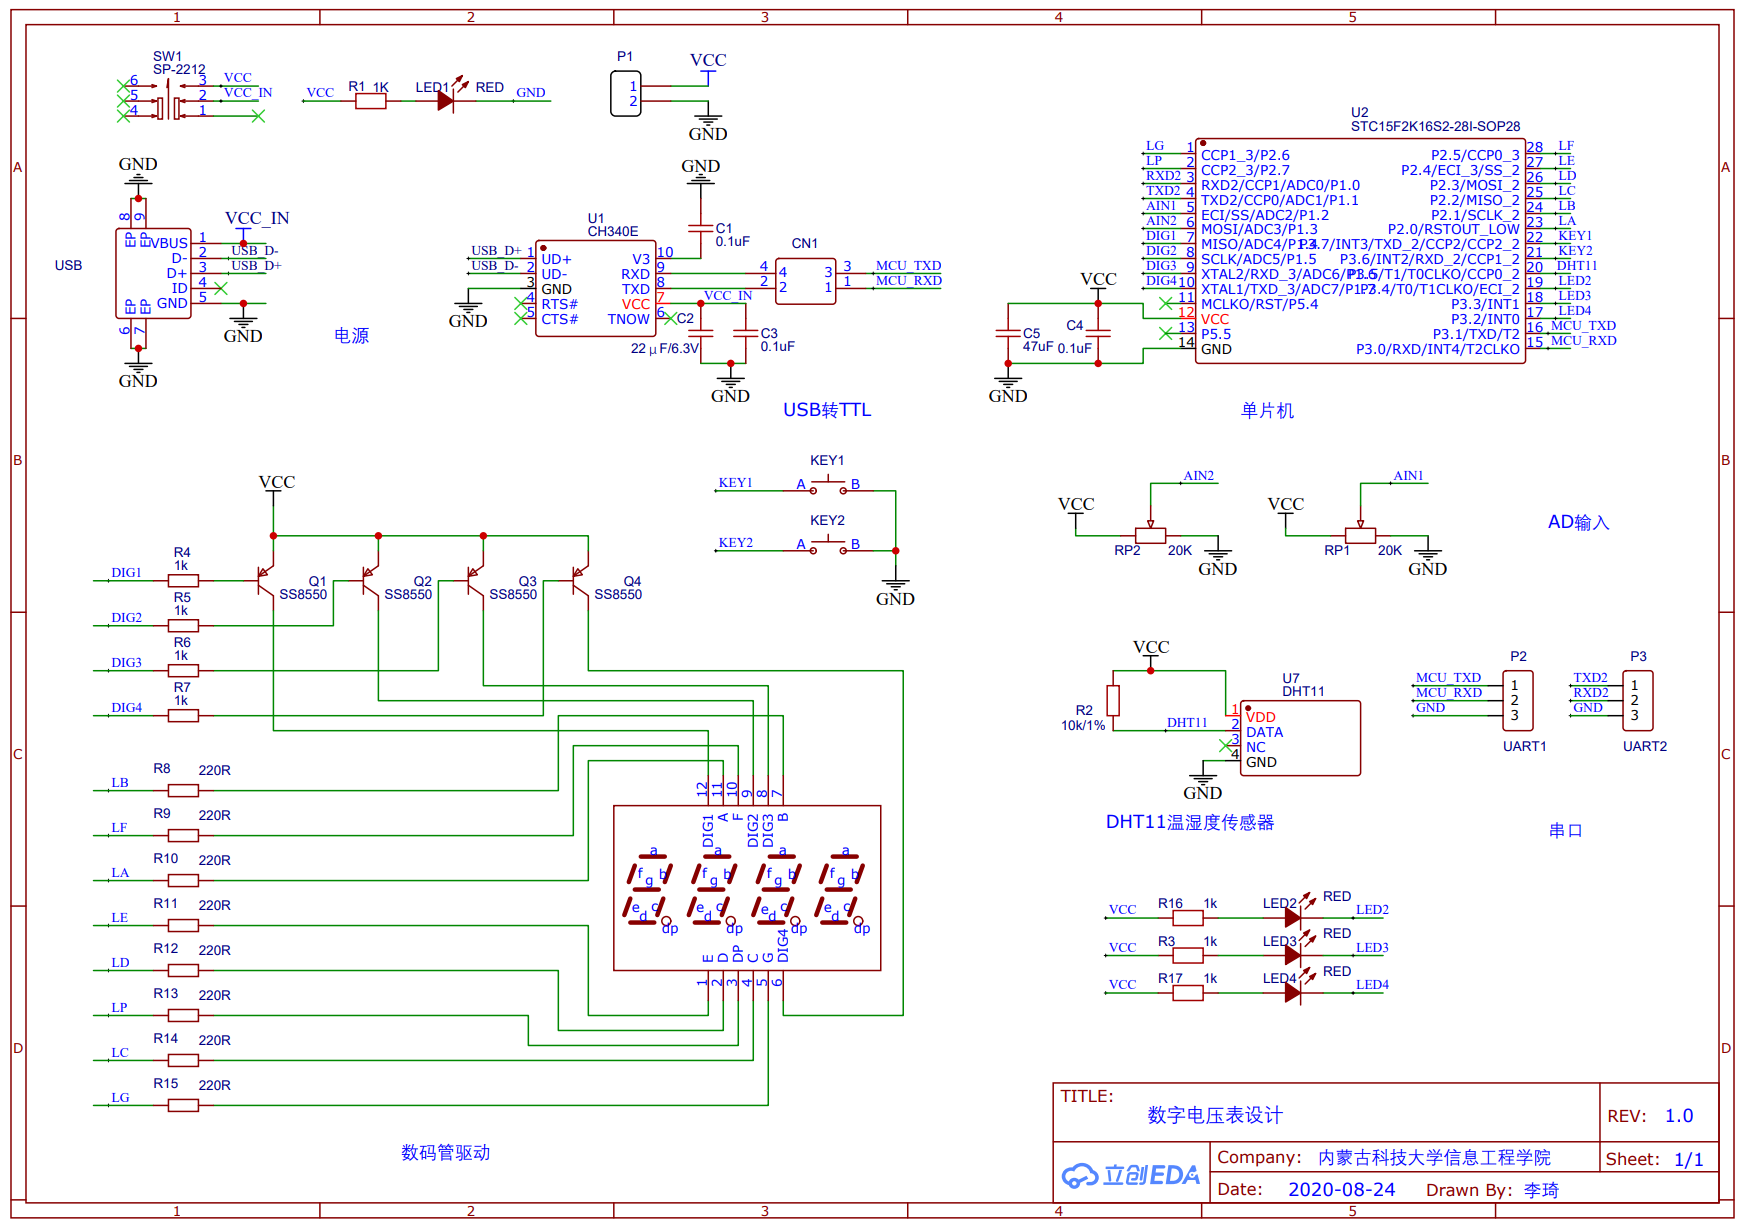
\includegraphics[width=\textwidth,angle=90]{figures/数字电压.png}
  \caption{单片机驱动四位数码管显示数字电压表电路原理图}
  \label{fig:5}
\end{figure}


\addtocontents{toc}{\protect\setcounter{tocdepth}{2}} % 恢复目录深度
\addcontentsline{toc}{chapter}{附录2}
\addtocontents{toc}{\protect\setcounter{tocdepth}{-1}} % 临时禁止加入目录
\chapter{}

这是一个关于数字电压表的源代码。这是一个关于数字电压表的源代码。这是一个关于数字电压表的源代码。这是一个关于数字电压表的源代码。这是一个关于数字电压表的源代码。这是一个关于数字电压表的源代码。

\begin{lstlisting}[language={[ANSI]C},extendedchars=false,tabsize=4, breaklines]
#include <reg51.h>
#include <intrins.h>
#include "common.h"
#define FOSC 11059200ul
#define T0_H (65536-(2*FOSC)/(1000*12))/256
#define T0_L (65536-(2*FOSC)/(1000*12))%256

sbit COM0 = P1^0;
sbit COM1 = P1^1;
sbit COM2 = P1^2;
sbit COM3 = P1^3;
sbit TLC549_CS = P1^6;
sbit TLC549_DOUT = P1^5;
sbit TLC549_CLK = P1^7;
bit flag = 0;
bit flag1 = 0;
uint8_t ADcounts = 0;
uint8_t dispBuf[] = { 2, 0, 1, 8};
uint8_t code ledDeg[] = { 0xC0, 0xF9, 0xA4, 0xB0, 0x99, 0x92, 0x82, 0xF8, 0x80, 0x90 };
uint8_t bdata AdValue;
sbit AIN = AdValue ^ 0;

void initSys();

uint8_t getAdValue() {
	uint8_t i;
	TLC549_CS = 0;
	TLC549_DOUT = 1;
	TLC549_CLK = 0;
	for (i = 0; i < 8; i++) {
		AdValue = AdValue << 1;
		TLC549_CLK = 1;
		_nop_();
		_nop_();
		AIN = TLC549_DOUT;
		TLC549_CLK = 0;
		_nop_();
		_nop_();
	}
	TLC549_CS = 1;
	return AdValue;
}

void main() {
	uint8_t i = 0;
	uint8_t j = 0;
	uint8_t ucAdValue = 0;
	uint16_t uiAdValue = 0;
	float fAdValue = 0.0;
	initSys();
	while (1) {
		if (flag1) {
			flag1 = 0;
			ucAdValue = getAdValue();
			fAdValue = (float)(ucAdValue * (5.0 / 255.0));
			uiAdValue = fAdValue * 1000;
			for (j = 0; j < 4; j++) {
				dispBuf[3 - j] = uiAdValue % 10;
				uiAdValue /= 10;
			}
		}
		if (flag) {
			flag = 0;
			switch (i) {
			case 0:
				COM0 = 0; COM1 = 1; COM2 = 1; COM3 = 1;
				break;
			case 1:
				COM0 = 1; COM1 = 0; COM2 = 1; COM3 = 1;
				break;
			case 2:
				COM0 = 1; COM1 = 1; COM2 = 0; COM3 = 1;
				break;
			case 3:
				COM0 = 1; COM1 = 1; COM2 = 1; COM3 = 0;
				break;
			}
			P3 = ledDeg[dispBuf[i]];
			if (i == 0)
				P3 &= 0x7f;
			if (++i >= 4)
				i = 0;
		}
	}
}

void initSys() {
	TMOD &= 0xF0;
	TMOD |= 0x01;
	EA = 1;
	ET0 = 1;
	TH0 = T0_H;
	TL0 = T0_L;
	TR0 = 1;
}

void timer0ISR()interrupt 1 {
	TH0 = T0_H;
	TL0 = T0_L;
	flag = 1;
	if (ADcounts++ >= 40) {
		ADcounts = 0;
		flag1 = 1;
	}
}
\end{lstlisting}  

\addtocontents{toc}{\protect\setcounter{tocdepth}{2}} % 恢复目录深度